\section[Long-term actions]{\Gls{longTermAct}}
\label{sec:example:tkm}


\subsection{Motivation}
\label{sec:tkm:intro:motiv}

\subsubsection{Delayed action}
\label{sec:tkm:intro:motiv:delayed_action}

In this section, we motivate the need to reason over delayed actions.
To do so, we first give four examples of these actions.
Then we detail why the effects of actions should be considered.
Finally, we summarise and motivate the need for incorporating actions and their effects on the knowledge. 

\paragraph{Delayed action examples}
Until here, we have claimed that adaptation processes should handle delayed actions.
In order to show their existence, we give four different examples: two based on our use case, one on cloud infrastructure and a last one on smart homes.
From our understanding, three phenomena can explain this delay: the time to execute an action(s) (Example 1), the time for the system to handle the new configuration (Example 3) and the inertia of the measured element (Example 2 and 4).

\subparagraph{Example 1: Modification of fuse states in smart grids}
Even if the Luxembourg power grid is moving to an autonomous one, not all the elements can be remotely controlled.
One example is fuses that still need to be open or closed by a human.
Open and close actions in the Luxembourg smart grid both imply technicians who are contacted, drive to fuse places and manually change their states.
If several fuses need to be changed due to one decision, only one technician will drive to them, sequentially, and executes the modifications.
For example, in our case, our industrial partner asks us to consider that each fuse modification takes 15 min whereas any incident should be detected in the minute.
Let's imagine that an incident is detected at 4 p.m. and can be solved by modifying three fuses.
The incidents will be seen as resolved by the adaptation process at 4 p.m. + 15 min * 3 = 4:45 p.m.
In this case, the delay of the action is due to the execution time that is not immediate.

\subparagraph[Example 2: Reduction of amps limits in smart grids]{Example 2: Reduction of amps limit in smart grids\footnote{This example is based on randomly generated data. As this action is not yet available on the Luxembourg smart grid, we miss real data. However, it reflects an hypothesis shared with our partner.}}
\begin{figure}
	\centering
	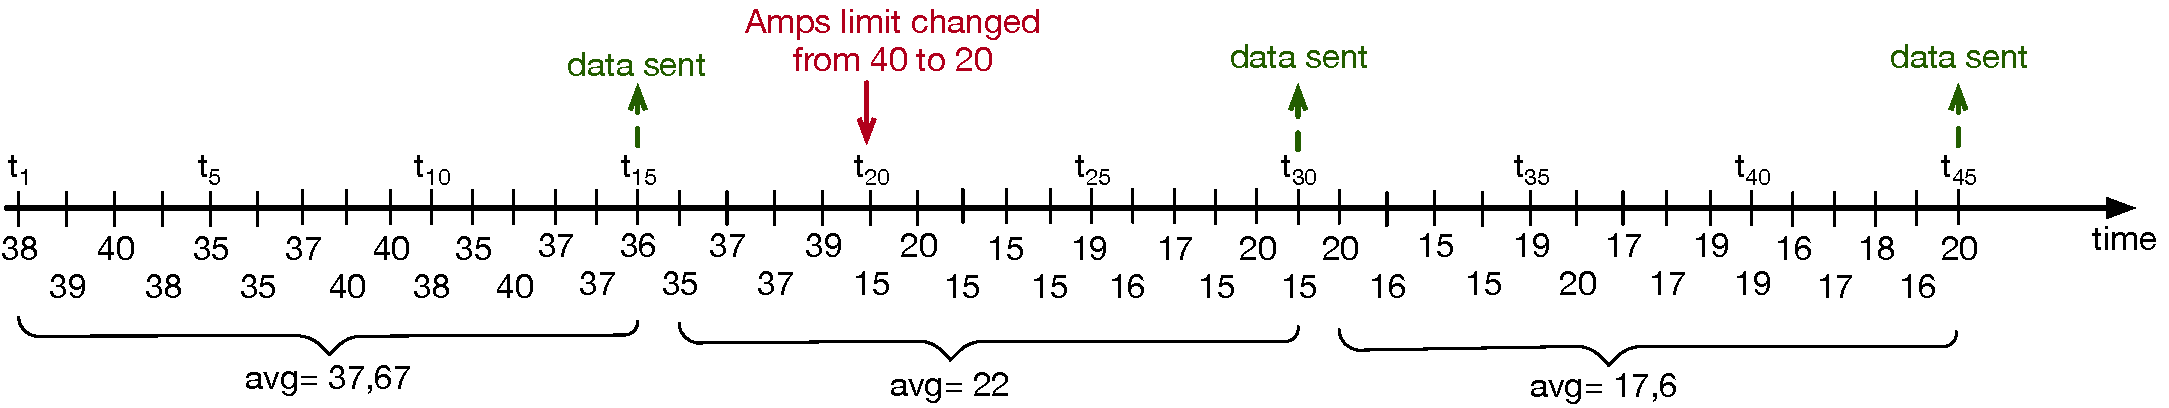
\includegraphics[width=\linewidth]{img/chapt-tkm/intro/long-action-amps-limit}
	\caption{Example of consumption measurement before and after a limitation of amps has been executed at $t_{20}$.}
	\label{fig:tkm:intro:example-long-action-amps-limit}
\end{figure}

In its smart grid project, \creos envisages controlling remotely amps limits of customers.
Customers will have two limits: a fixed one, set at the beginning, and a flexible one, remotely managed.
The action to remotely change amps limits will be performed through specific plugs, such as one for electric vehicles.
Even if the action is near instant, due to how power consumption is collected, its impacts would not be visible immediately.
Indeed, data received by \creos corresponds to the total energy consumed since the installation.
From this information, only the average of consumed data for the last period can be computed.

In Figure~\ref{fig:tkm:intro:example-long-action-amps-limit}, we depict a scenario that shows the delay between the action is executed and the impacts are measured.
Each time point represents one minute, with the consumption at this moment.

Let's imagine a customer who has his or her limit set to 40 amps\footnote{The user cannot consume more than 40 amps at a precise time $t_i$.} and consumes near this limit.
We consider that data are sent every 15 min.
After receiving data sent $t_{15}$ and processing them, the adaptation process detects an overload and decides to reduce the limits to 20 amps for the customer.
However, considering the delay for data to be collected and the one to send data\footnote{Reminder: the smart grid is not built upon a fast network such a fiber network.}, the action is received and executed at $t_{20}$.
At $t_{30}$, new consumption data is sent, here equals 22 amps.
Here, there are two situations.
First, this reduction was enough to fix the overload.
Even in this idealistic scenario, the adaptation process must wait at worst 15 min ($t_{30}$ - $t_{15}$) to see the resolution (without considering the communication time).
Second, this reduction was not enough - as the adaptation process considered that the consumption data will be at worst 20 amps and here it is 22.
Before seeing the incident as solved and knowing that the decision fixed the incident, the adaptation process should wait for new data, sent at $t_{45}$, \ie around 30 min ($t_{45} - t_{15}$) after the detection.

In this case, the delay of this action can be explained by the inertia in the average of the consumption.

\subparagraph{Example 3: Switching off a machine from a load balancer}
\begin{figure}
	\centering
	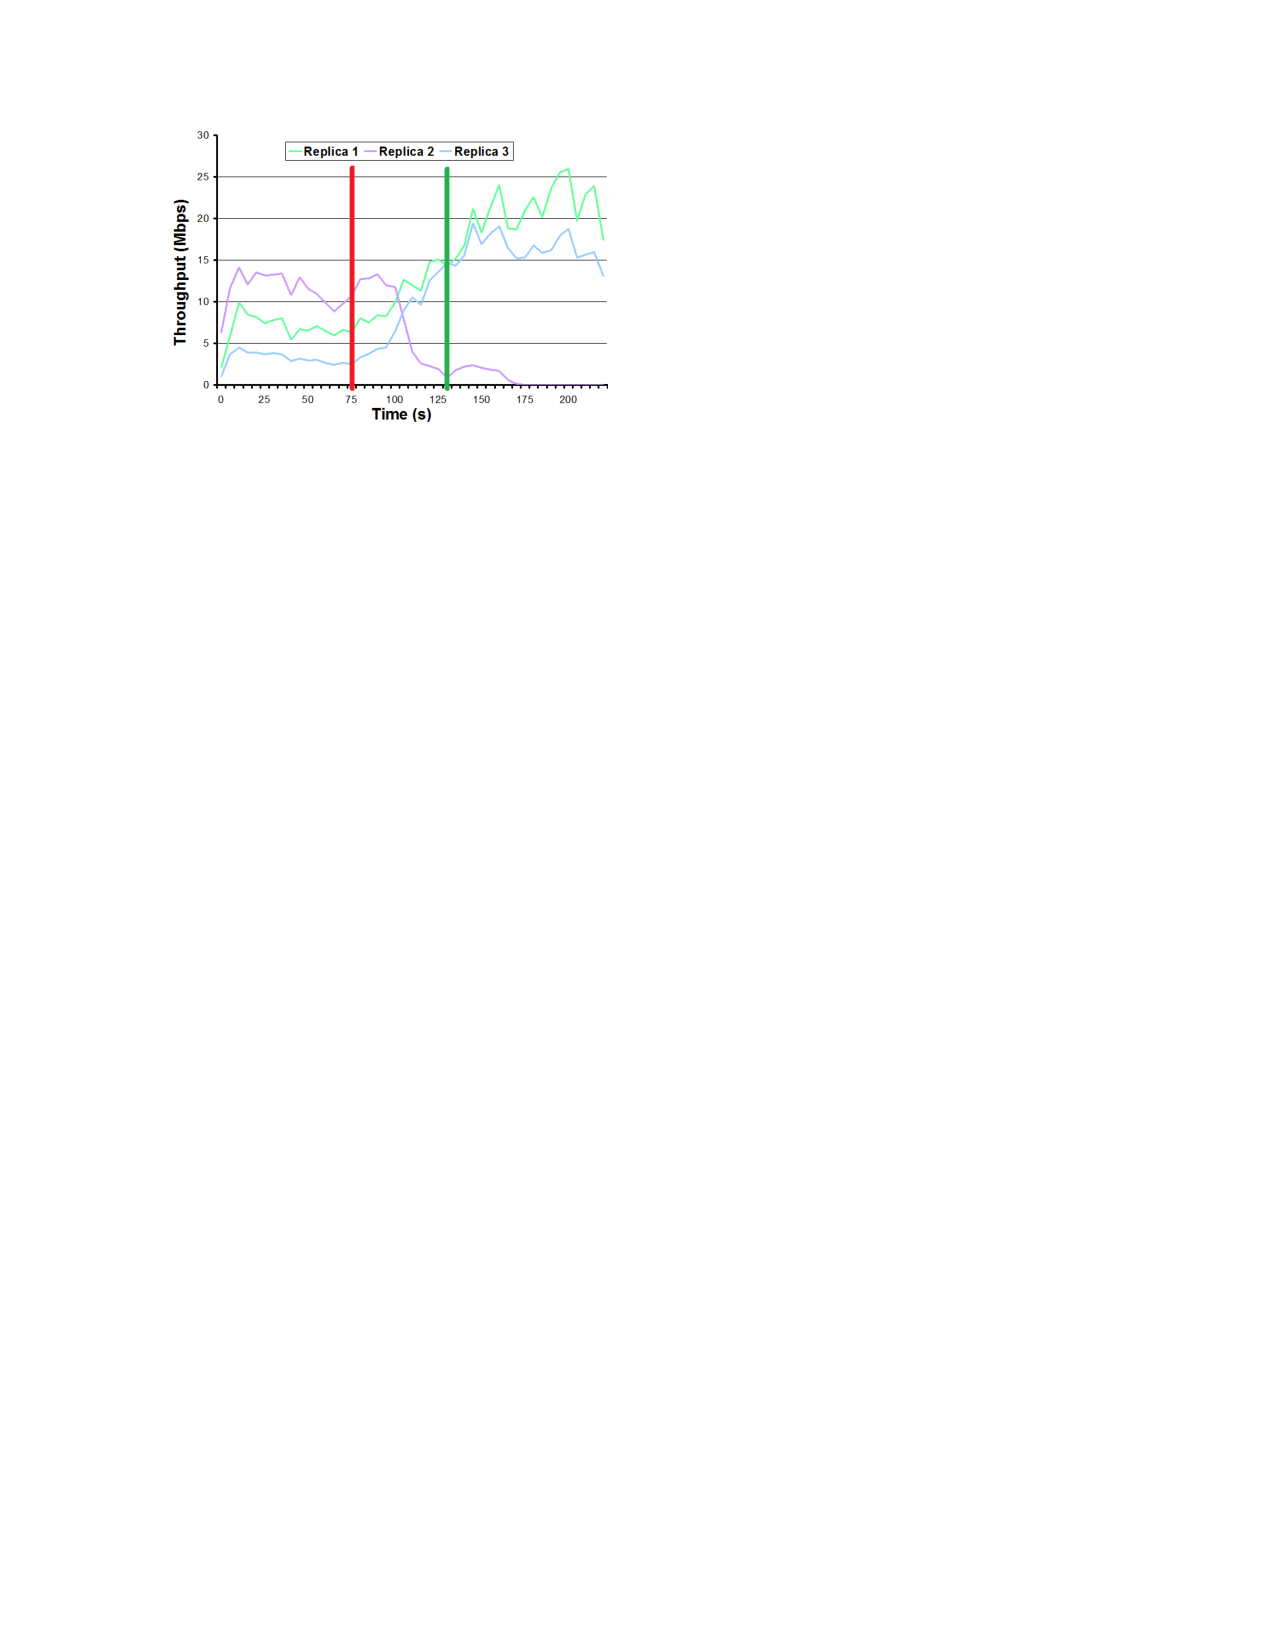
\includegraphics[width=0.5\linewidth]{img/chapt-tkm/intro/load-balencer}
	\caption{Figure extracted from~\cite{DBLP:conf/nsdi/WangBR11}. The red bar depicted the moment when Replica 2 stop receiving new connections. The green one represents the moment where all the rules in the load balancer stop considering R2. Despite these two actions, the throughput of the machine does not drop to 0 due to existing and active connections.}
	\label{fig:tkm:intro:example-load-balencer}
	
\end{figure}


An example based on cloud infrastructure of delayed actions is to remove a machine from a load balancer, for example during a scale down operation.
Scale down operations allows cloud managers to reduce allocated resources for a specific task.
It is used either to reduce the cost of the infrastructure or to reallocate them to other tasks.
In~\cite{DBLP:conf/nsdi/WangBR11}, Wang~\etal present a load-balancing algorithm.
In their evaluation, they present the figure depicted in Figure~\ref{fig:tkm:intro:example-load-balencer} that shows the evolution of the throughput after the server Replica 2 (R2) is removing from the load balancer.
The red bar shows the moment where R2 stop receiving new connection and the green the moment where it is removed from the load balancer algorithm.
However, despite these actions have been taken, R2 should finish the ongoing tasks that it is executing.
This explains why the throughout is progressively decreasing to 0 and there is a delay of around 100s between the red bars and the moment where R2 stop being active.

This example shows a delayed action due to the time required by the system to handle the new configuration.

\subparagraph{Example 4: Modifying home temperature through a smart home system}
Smart home systems have been implemented in order to manage remotely a house or to perform automatically routines.
For example, it allows users to close or open blinds from their smartphones.
Based on instruction temperatures, smart home systems manage the heating or cooling system to reach them at the desired time.
However, heating or cooling a house is not immediate, it can take several hours before the targeted temperature is reached.
Plus, if the temperature sensor and the heating or cooling system are not placed nearby, the new temperature can take time before being measured.
This can be explained due to the temperature inertia plus the delay for the temperature to be propagated.

\bigskip

Through these four examples, we show that delayed actions can be found in different kinds of systems, from CPS to cloud infrastructure.
However, not only knowing that an action is running is important but also knowing its expecting effect.
We detail this point in the following section.

\paragraph{The need to consider effects}
In the previous section, we show the existence of delayed actions.
One may argue that action statuses are already integrated into the knowledge.
For example, the OpenStack Watcher framework stores them in a database\footnote{\url{https://docs.openstack.org/watcher/latest/glossary.html\#watcher-database-definition}}, accessible through an API.
However, for the best of our knowledge Watcher does not store the expecting effects of each action.
While the adaptation process knows what action is running, it does not know what it should expect from them.

Considering our example based on the modification of fuses, if the system knows that the technician is modifying fuse states, it does not know what would be the effects.
In this case, when the adaptation process analyses the system context it may wonder: what will be the next grid configuration? How the load will be balanced? Will the future configuration fix all the current incidents?
If the effects are not considered by the adaptation process, then it may take suboptimal decisions.

Let's exemplify this claim through a scenario based on the fuse example (\cf Example 1).
As explained before, the overload detected at 4 p.m. takes around 45 min to be fixed.
The system marks this incident as \textquote{being resolved}.
In addition to this information, the knowledge contains another one saying that it is being solved by modifying three fuses.
However, during the resolution stage, a cable is also being overloaded.
The adaptation process has two solutions.
It can either wait for the end of the resolution of the first incident to see if both overloaded elements will be fixed or it takes other actions without considering the ongoing actions and their impacts.
Applying the first strategy may make the resolution of the second incident late, whereas the second one may generate a suboptimal sequence of actions.
For example, the second modifications may undo what has been done before or both actions may be conflicting.

\paragraph{Conclusion}
Actions, like fuse modification in a smart grid or removing a server from a load balancer, generated during by adaptation processes could take time upon completion. 
Moreover, the expected effects resulting from such action is reflected in the context representation only after a certain delay. 
One used workaround is the selection, often empirically, of an optimistic time interval between two iterations of the MAPE-K loop such that this interval is bigger than the longest action execution time.
However, the time to execute an action is highly influenced by system overload or failures, making such empirical tuning barely reliable.
We argue that by enriching context representation with support for past and future planned actions and their expected effects over time, we can highly enhance reasoning processes and avoid empirical tuning.

The research question that motivates our work is thus: how to enable reasoning over unfinished actions and their expected effects?

Fined and rich context information directly influences the accuracy of the actions taken.
Various techniques to represent context information have been proposed; among which we find the models@run.time~\cite{DBLP:journals/computer/MorinBJFS09, DBLP:journals/computer/BlairBF09}.
The models@run.time \linebreak paradigm inherits model-driven engineering concepts to extend the use of models not only at design time but also at runtime. 
This model-based representation has proven its ability to structure complex systems and synthesize its internal state as well as its surrounding environment.

\subsubsection{Diagnosis support}

Faced with growingly complex and large-scale software systems (e.g. smart grid systems), we can all agree that the presence of residual defects becomes unavoidable~\cite{DBLP:conf/icse/BarbosaLMJ17, DBLP:conf/icse/MongielloPS15, DBLP:conf/icse/HassanBB15}. 
Even with a meticulous verification or validation process, it is very likely to run into an unexpected behaviour that was not foreseen at design time. Alone, existing formal modelling and verification approaches may not be sufficient to anticipate these failures~\cite{DBLP:conf/icse/TaharaOH17}. 
As such, complementary techniques need to be proposed to locate the anomalous behaviour and its origin in order to handle it in a safe way.

As there might be many probable causes behind an abnormal behaviour, developers usually perform a set of diagnosis routines to narrow down the scope or origin of the failure. One way to do so is by investigating the satisfaction of its requirements and the decisions that led to this system state, as well as their timing~\cite{DBLP:conf/iceccs/BencomoWSW12}.  
In this perspective, developers may set up a set of systematic questions that would help them understand why and how the system is behaving in such a way.
These questions may comprise: 
\begin{itemize}
   \item what goal(s) the system was trying to reach by executing a tactic $a$? 
   \item what were the circumstances used by a decision $d$ and its expected impact on the context?
   \item what decision(s) influenced the system's context at a time $t$? 
\end{itemize}

Bencomo~\etal~\cite{DBLP:conf/iceccs/BencomoWSW12} argue that comprehensive explanation about the system behaviour contributes drastically to the quality of the diagnosis, and eases the task of troubleshooting the system behaviour.
To enable this, we believe that adaptive software systems should be equipped with traceability management facilities to link the decisions made to their \textbf{(i) circumstances, that is to say, the history of the system states and the targeted requirements, and (ii) the performed actions with their impact(s) on the system}.
In particular, an \textbf{adaptive system should keep a trace of the relevant historical events}.
Additionally, it should be able to \textbf{trace the goals intended to be achieved by the system to the adaptations and the decisions that have been made, and vice versa}. 
Finally, in order to enable developers to interact with the system in a clear and understandable way, appropriate abstraction to \textbf{enable the navigation of the traces and their history should also be provided}.
Unfortunately, suitable solutions to support these features are under-investigated. 

Existing approaches~\cite{hassel13,DBLP:conf/models/HeinrichSJRMHRP14,DBLP:conf/icac/EhlersHWH11,DBLP:conf/icse/MendoncaAR14,DBLP:conf/icse/CasanovaGSA14,DBLP:conf/icse/IftikharW14a} are accompanied by built-in monitoring rules and do not allow to interact with the underlying system in a simple way. 
Moreover, they do not keep track of historical changes as well as causal relationships linking requirements to their corresponding adaptations. Only flat execution logs are stored. 

\subsection{Use case scenario}
\label{sec:tkm:intro:uc}

\begin{figure}
	\centering
	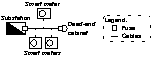
\includegraphics[width=0.5\linewidth]{img/chapt-tkm/formalism/excerptSG}
	\caption{Simplified version of a smart grid}
	\label{fig:tkm:excerptSG}
\end{figure}

In order to provide a readable and understandable example of the formalism, we give a simplified version of the use case presented in Section~\ref{sec:intro:use-case}.

\paragraph{Excerpt of a smart grid}
Figure~\ref{fig:tkm:excerptSG} shows a simplified version of a smart grid with one substation, one cable, three smart meters and one dead-end cabinet.
Both the substation and the cabinet have one fuse each.
The meters regularly send consumption data at the same timestamp.
For this example, we consider one requirement: minimizing the number of overloads.
To achieve so, among the different actions, two actions are taken into account in this example: decreasing or increasing the amps limits of smart meters.

\paragraph{Adaptation scenario}
The system starts at $t_0$ with the actions, the requirements and all element of the context that remain fixed: the grid installation.
Meters send their values at $t_1$, $t_2$ and $t_3$.
Based on these data, the load on cables and substation is computed.
On $t_1$, an overload is detected on the cable, which breaks the requirement.
At the same time point, the system decides to reduce the load of all smart meters.
The impact of these actions will be measured at $t_2$ and $t_3$, \ie the consumption will slowly reduce until the cable is no longer overloaded from $t_3$.

\paragraph{Diagnosis scenario}
As all adaptive systems, smart grids are prone to \linebreak failures~\cite{DBLP:conf/smartgridsec/0001FKNT14}.
Using our approach, an engineer could diagnose the system, and determine the adaptation process responsible for this failure. 
For instance, considering some reports about regular power cuts during the last couple of days, in a particular area, a stakeholder may want to interrogate the system and determine what past decision(s) have led to this suboptimal state.
More concretely, he will ask: did the system make any decisions that could have impacted the customer consumption? 
If so, what goal(s) the system was trying to reach and what were the values used at the time the decision(s) was(were) made?